\renewcommand{\theequation}{\theenumi}
\begin{enumerate}[label=\arabic*.,ref=\thesection.\theenumi]
\numberwithin{equation}{enumi}
%
%
\item  An object travels 16m in 4s and then another 16 m in 2 s. What is the average speed of the object?
\item  The odometer of a car reads 2000 km at the start of a tri and 2400 km at the end of the trip.  If the trip took 8 h, calculat the average speed of the car in km/h and m/s.
\item  Usha swims in a 90m long pool.  She covers 180m in one minute by swimming from one end to the other and back along the same straight path.  Find the average speed and average velocity of Usha.
\item  Starting from a stationary position, Rahul paddles his bicycle to
attain a velocity of $6 m s^{-1}$ in $30 s$. Then
he applies brakes such that the velocity of the bicycle comes down to $4 m s^{-1}$
the next $5 s$. Calculate the acceleration of the bicycle in both the cases
%
\item  A train starting from rest attains a velocity of $72 km h^{-1}$
in
5 minutes. Assuming that the acceleration is uniform, find (i) the acceleration and (ii) the distance travelled by the train for attaining this velocity.
%
\item  A car accelerates uniformly from $18 km h
^{-1}$ to $36 km h^{-1}$ in $5 s$. 
Calculate 
\begin{enumerate}
\item  the acceleration and 
\item   the distance covered by the car in that time.
\end{enumerate}
%
\item  The brakes applied to a car produce an acceleration of $6 m s^{-2}$
in
the opposite direction to the motion. If the car takes $2 s$ to stop after the application of brakes, calculate the distance it travels during this time.
%
\item  A constant force acts on an object of mass 5 kg for a duration of 2 s. It increases the object’s velocity from 3 $m s^{-1}$
to 7 $m s^{-1}$ . Find the
magnitude of the applied force. Now, if the force was applied for a duration of 5 s, what would be the final velocity of the object?
\item  Which would require a greater force -- accelerating a 2 kg mass at 5 $m s^{-2}$
or a 4 kg mass at 2 $m s^{-2}$?
\item  A motorcar is moving with a velocity of 108 km/h and it takes 4 s to stop after the brakes are applied. Calculate the force exerted by the brakes on the motorcar if its mass along with the passengers is 1000 kg.
\item  A force of 5 N gives a mass m1
, an acceleration of 10 $m s^{-2}$ mass m2, an acceleration of 20 $m s^{-2}$
and a .
What acceleration would it give if both the masses were tied together?
\item  A bullet of mass 20 g is horizontally fired with a velocity 150 $m s^{-1}$
What is the recoil velocity of the pistol?
\item  A girl of mass 40 kg jumps with a horizontal velocity of 5 $m s^{-1}$
onto
a stationary cart with frictionless wheels. The mass of the cart is 3 kg. What is her velocity as the cart starts moving? Assume that there is no external unbalanced force working in the horizontal direction.
\item  Two hockey players of opposite teams, while trying to hit a hockey ball on the ground collide and immediately become entangled. One has a mass of 60 kg and was moving with a velocity 5.0 $m s^{-1}$
while the other
has a mass of 55 kg and was moving faster with a velocity 6.0 $m s^{-1}$
towards
the first player. In which direction and with what velocity will they move after they become entangled? Assume that the frictional force acting between the feet of the two players and ground is negligible.

\item  The mass of the earth is 6 $\times$ 1024
kg. If the distance between the earth and the moon is 3.84$\times$105
7.4 $\times$ 1022
calculate the force exerted by the earth on the moon. (Take G = 6.7 $\times 10^{-11}
N m^2$ 
\item  A car falls off a ledge and drops to the ground in 0.5 s. 
\begin{enumerate}
\item   What is its speed on striking the ground?
\item   What is its average speed during the 0.5 s?
\item   How high is the ledge from the ground?
\end{enumerate}
Let $g = 10 m s^{-2}$.
\item  An object is thrown vertically upwards and rises to a height of 10 m. Calculate (i) the velocity with which the object was thrown upwards and (ii) the time taken by the object to reach the highest point. Let $g = 9.8 m s^{-2}$.
\item  Mass of an object is 10 kg. What is its weight on the earth?
\item  An object weighs 10 N when measured on the surface of the earth. What would be its weight when measured on the surface of the moon?
\item  A block of wood is kept on a tabletop. The mass of wooden block is 5 kg and its dimensions are 40 cm $\times$ 20 cm $\times$ 10 cm. Find the pressure exerted by the wooden block on the table top if it is made to lie on the table top with its sides of dimensions (a) 20 cm $\times$ 10 cm and (b) 40 cm $\times$ 20 cm.
\item  Relative density of silver is 10.8. The density of water is $103
kg m^{-3}$.  What is the density of silver in SI unit? 
\item  A force of 7 N acts on an object. The displacement is, say 8 m, in the direction of the force. Let us take it that the force acts on the object through the displacement. What is the work done in this case?
\item  A porter lifts a luggage of 15 kg from the ground and puts it on his head 1.5 m above the ground. Calculate the work done by him on the luggage.
\item  An object of mass 15 kg is moving with a uniform velocity of 4
$m s^{-1}$ 
. What is the kinetic energy possessed by the object?
\item  What is the work to be done to increase the velocity of a car from 30 $km h^{-1}$
to 60 $km h^{-1}$ the car is 1500 kg? 
\item  The kinetic energy of an object of mass, m moving with a velocity of 5 $m s^{-1}$
is 25 J. What will be its
kinetic energy when its velocity is doubled? What will be its kinetic energy when its velocity is increased three times?
\item   Find the energy possessed by an object of mass 10 kg when it is at a height of 6 m above the ground. Given, g = 9.8 $m s^{-2}$
.
\item  An object of mass 12 kg is at a certain height above the ground. If the potential energy of the object is 480 J, find the height at which the object is with respect to the ground. Given, g = 10 $m s^{-2}$.
\item  Two girls, each of weight 400 N climb up a rope through a height of 8 m. We name one of the girls A and the other B. Girl A takes 20 s while B takes 50 s to accomplish this task. What is the power expended by each girl?
\item  A boy of mass 50 kg runs up a staircase of 45 steps in 9 s. If the height of each step is 15 cm, find his power. Take g = 10 $m s^{-2}$
.
\item  An electric bulb of 60 W is used for 6 h per day. Calculate the 'units' of energy consumed in one day by the bulb.
\item  A sound wave has a frequency of 2 kHz and wave length 35 cm. How long will it take to travel 1.5 km?
\item  A person clapped his hands near a cliff and heard the echo after 2 s. What is the distance of the cliff from the person if the speed of the sound, v is taken as 346 $m s^{-1}$?
\item  A ship sends out ultrasound that returns from the seabed and is
detected after 3.42 s. If the speed of ultrasound through seawater is 1531 m/s, what is the distance of the seabed from the ship?
\item  A convex mirror used for rear-view on an automobile has a radius of curvature of 3.00 m. If a bus is located at 5.00 m from this mirror, find the position, nature and size of the image.
\item  An object, 4.0 cm in size, is placed at 25.0 cm in front of a concave mirror of focal length 15.0 cm. At what distance from the mirror should a screen be placed in order to obtain a sharp image? Find the nature and the size of the image.
\item  A concave lens has focal length of 15 cm. At what distance should the object from the lens be placed so that it forms an image at 10 cm from the lens? Also, find the magnification produced by the lens.
\item  A 2.0 cm tall object is placed perpendicular to the principal axis of a convex lens of focal length 10 cm. The distance of the object from the lens is 15 cm. Find the nature, position and size of the image. Also find its magnification.
\item  A current of 0.5 A is drawn by a filament of an electric bulb for 10 minutes. Find the amount of electric charge that flows through the circuit.
\item  How much work is done in moving a charge of 2 C across two points having a potential difference 12 V?
\item  
\begin{enumerate}
\item  How much current will an electric bulb draw from a 220 V source, if the resistance of the bulb filament is 1200 $\ohm$?
\item   How much current will an electric heater coil draw from a 220 V source, if the resistance of the heater coil is 100 $\ohm$?
\end{enumerate}
\item  The potential difference between the terminals of an electric heater is 60 V when it draws a current of 4 A from the source. What current will the heater draw if the potential difference is increased to 120 V?
\item  Resistance of a metal wire of length 1 m is 26 $\ohm$ at 20$\degree$C. If the diameter of the wire is 0.3 mm, what will be the resistivity of the metal at that temperature? Predict the material of the wire.
\item  A wire of given material having length l and area of cross-section A has a resistance of 4 $\ohm$. What would be the resistance of another wire of the same material having length l/2 and area of cross-section 2A?
\item  An electric lamp, whose resistance is 20 $\ohm$, and a conductor of 4 $\ohm$ resistance are connected in series to a 6 V battery . Calculate (a) the total resistance of the circuit, (b) the current through the circuit, and (c) the potential difference across the electric lamp and conductor.
\item  Resistors R1 R2 and R3 connected in parallel, have the values 5 $\ohm$, 10 $\ohm$, 30 $\ohm$, respectively, which have been connected to a battery of 12 V. Calculate 
%
\begin{enumerate}
\item   the current through each resistor, 
\item   the total current in the circuit, and 
\item   the total circuit resistance.
\end{enumerate}
\item  If in Fig. \ref{fig:ckt_class10},
R1= 10 $\ohm$, R2 = 40 $\ohm$, R3 = 30 $\ohm$, R4 = 20 $\ohm$, R5 = 60 $\ohm$,
and a 12 V battery is connected to the arrangement. Calculate 
%
\begin{enumerate}
\item  the total resistance in the circuit, and 
\item  the total current flowing in the circuit.
\end{enumerate}

\begin{figure}[!ht]
\centering
\includegraphics[width=\columnwidth]{./figs/ckt.eps}
\caption{}
\label{fig:ckt_class10}
\end{figure}
\item  An electric iron consumes energy at a rate of 840 W when heating is at the maximum rate and 360 W when the heating is at the minimum. The voltage is 220 V. What are the current and the resistance in each case?
\item  100 J of heat is produced each second in a 4 $\ohm$ resistance. Find the potential difference across the resistor.
\item  An electric bulb is connected to a 220 V generator. The current is 0.50 A. What is the power of the bulb?
\item  An electric refrigerator rated 400 W operates 8 hour/day. What is the cost of the energy to operate it for 30 days at Rs 3.00 per kW h?
\item  A car is moving along a straight line, say OP. It moves from O to P in 18 s and returns from P to Q in 6.0 s. What are the average velocity and average speed of the car in going 
\begin{enumerate}
\item  from O to P ? and 
\item  from O to P and back to Q ?
\end{enumerate}
\item The position of an object moving along x-axis is given by $x = a + bt^2$ where $a = 8.5 m, b = 2.5 m s^{-2}$ and t is
measured in seconds.  What is the average velocity between t = 2.0 s and t = 4.0 s ?
\item  A ball is thrown vertically upwards with a velocity of 20 $ms^{-1}$ from the top of a multistorey building. The height of the point from where the ball is thrown is 25.0 m from the ground. 
\begin{enumerate}
\item  How high will the ball rise ? and 
\item  how long will it be before the ball hits the ground?
\end{enumerate} 
Take g = 10 $ms^{-2}$.
\item Two parallel rail tracks run north-south. Train A moves north with a speed of 54 $km h^{-1}$
with a speed of 90 $km h^{-1}$
, and train B moves south . What is the
\begin{enumerate}
\item  velocity of B with respect to A ?, 
\item  velocity of ground with respect to B ?, and
\item  velocity of a monkey running on the roof of the train A against its motion (with a velocity of 18 $km h^{-1}$
with
respect to the train A) as observed by a man standing on the ground ?
\end{enumerate}
\end{enumerate}
